%%%%%%%%%%%%%%%%%%%%%%%%%%%%%%%%%%%%%%%
% PlushCV - One Page Two Column Resume
% LaTeX Template
% Version 1.0 (11/28/2021)
%
% Author:
% Shubham Mazumder (http://mazumder.me)
%
% Hacked together from:
% https://github.com/deedydas/Deedy-Resume
%
% IMPORTANT: THIS TEMPLATE NEEDS TO BE COMPILED WITH XeLaTeX
%
%
%%%%%%%%%%%%%%%%%%%%%%%%%%%%%%%%%%%%%%
%
% TODO:
% 1. Figure out a smoother way for the document to flow onto the next page.
% 3. Add more icon options
% 4. Fix hacky left alignment on contact line
% 5. Remove Hacky fix for awkward extra vertical space
%
%%%%%%%%%%%%%%%%%%%%%%%%%%%%%%%%%%%%%%
%
% CHANGELOG:
%
%%%%%%%%%%%%%%%%%%%%%%%%%%%%%%%%%%%%%%%
%
% Known Issues:
% 1. Overflows onto second page if any column's contents are more than the vertical limit.
%%%%%%%%%%%%%%%%%%%%%%%%%%%%%%%%%%%%%%
%%Icons:
%%Main: https://icons8.com/icons/carbon-copy
%%%%%%%%%%%%%%%%%%%%%%%%%%%%%%%%%%

\documentclass[]{plushcv}
\usepackage{fancyhdr}
\usepackage{enumitem}
\pagestyle{fancy}
\fancyhf{}
\begin{document}

\setlist[itemize]{leftmargin=*}

%%%%%%%%%%%%%%%%%%%%%%%%%%%%%%%%%%%%%%
%
%     TITLE NAME
%
%%%%%%%%%%%%%%%%%%%%%%%%%%%%%%%%%%%%%%

% \hfill\smash{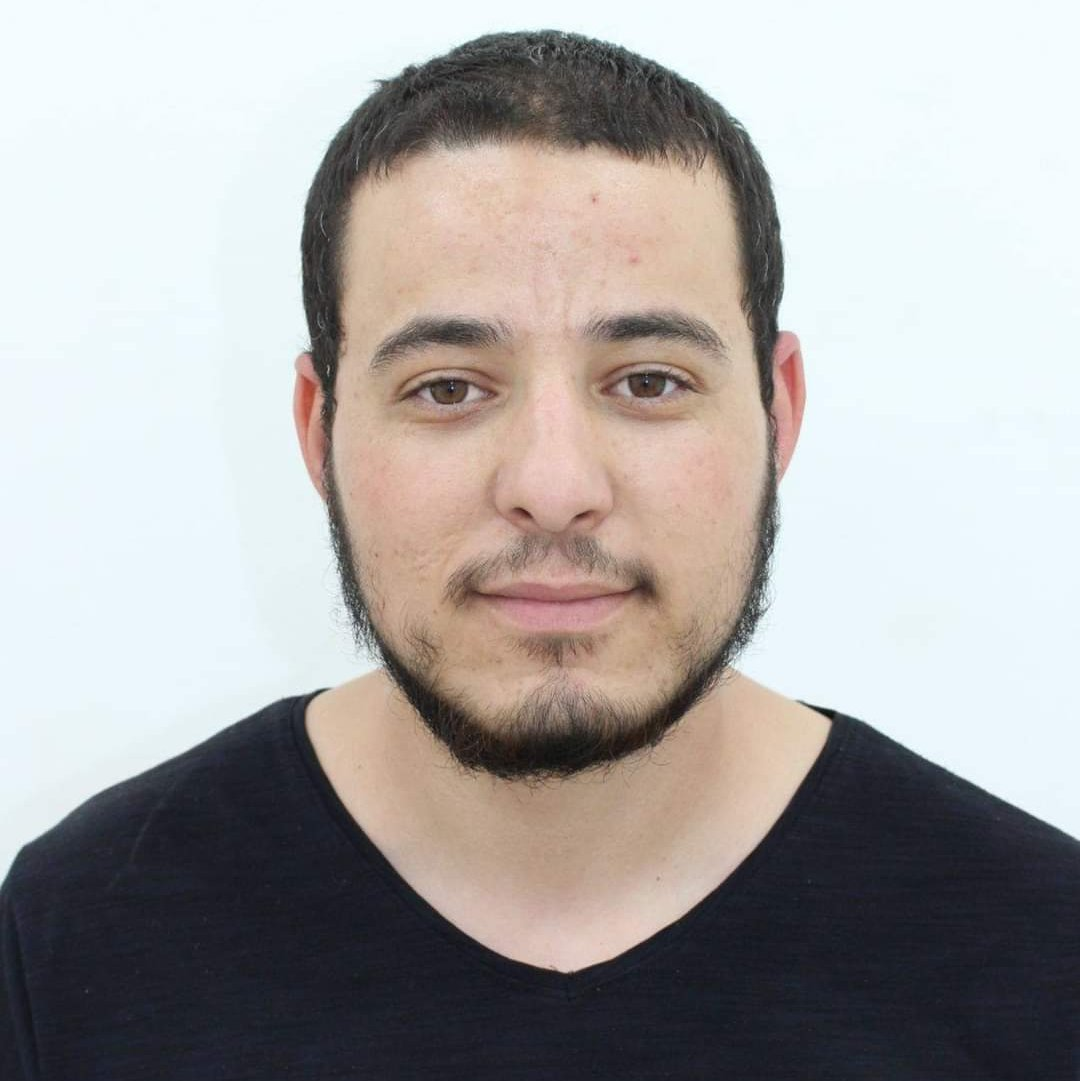
\includegraphics[width=2.5cm]{me.jpg}}
\small {
\namesection{Haroune}{Mohammedi}{Senior Data Engineer}{\small\contactline{Paris}{\href{https://www.github.com/mohammedi-haroune}{GitHub}}{\href{https://www.linkedin.com/in/haroune-mohammedi-3b3836170/}{LinkedIn}}{\href{mailto:mohammedi.haroun@gmail.com}{mohammedi.haroun@gmail.com}}{\href{tel:+33626850080}{0626850080}}{\href{https://haroune.me}{haroune.me}}}
}

% \vspace{2pt}
% \sectionsep
% \sectionsep
% \sectionsep

% \section{Introduction}
\vspace{16pt}

%Senior Data Engineer
Specialized in large-scale distributed data pipelines on Databricks/PySpark, currently at Engie, processing 50M+ rows/day of high-frequency data, optimizing workloads (up to 90\%) and migrating legacy Oracle ETL workflows. Operates across the full project lifecycle, from functional analysis and architecture design to deployment and production support. Strong focus on understanding domain challenges and bridging the gap between technical implementation and business needs.

\vspace{-6pt}

% \namesection{Firstname}{Lastname}{Full Stack Software Engineer}{\contactline{\href{https://www.mazumder.me}{mazumder.me}}{\href{https://www.github.com/sansquoi}{sansquoi}}{\href{https://www.linkedin.com/mazumders}{mazumders}}{\href{mailto:shubham.mazumder@gmail.com}{first.last@email.com}}{\href{tel:+1999999999}{9999999999}}}

%%%%%%%%%%%%%%%%%%%%%%%%%%%%%%%%%%%%%%
%
%     COLUMN ONE
%
%%%%%%%%%%%%%%%%%%%%%%%%%%%%%%%%%%%%%%

\begin{minipage}[t]{0.74\textwidth}


%%%%%%%%%%%%%%%%%%%%%%%%%%%%%%%%%%%%%%
%     EXPERIENCE
%%%%%%%%%%%%%%%%%%%%%%%%%%%%%%%%%%%%%%

\section{Experience}

\runsubsection{Engie}
\descript{| Senior Data Engineer }
\hfill
\location{Feb 2024 – Present | Paris, France}
% \hspace{10pt}
\vspace{\topsep} % Hacky fix for awkward extra vertical space
\begin{tightemize}
\sectionsep
\item Designed and implemented large-scale data pipelines processing 50M+ rows/day of high-frequency energy consumption data (30-min intervals) on Databricks/PySpark.

\item Migrated legacy ETL workflows from PL/SQL to PySpark on Databricks, reducing execution time from several weeks to a few hours and generating substantial compute cost savings.

\item Optimized PySpark pipelines achieving 90\%+ performance improvement (10 hours → under 1 hour) through Spark tuning, partitioning strategies, and scalable architecture design.

\item Led projects end-to-end: functional analysis, architecture design, development, testing, deployment (MEP), and production support (RUN).

\item Developed strong functional expertise in the energy domain, with a genuine interest in business challenges and operational processes.

\item Ensured data quality and reliability of production pipelines in a critical context.
\end{tightemize}
\sectionsep
\sectionsep


\runsubsection{Quadratic}
\descript{| Senior Data Engineer }
\hfill
\location{May 2022 – Jan 2024 | Paris, France}
% \hspace{10pt}
% \vspace{\topsep} % Hacky fix for awkward extra vertical space
\vspace{5pt}
\begin{tightemize}
\sectionsep
\item Designed and implemented a real-time blockchain data integration pipeline, synchronizing on-chain events from Web3 smart contracts into MongoDB, making blockchain data accessible to Web2 applications.
\item Designed the MongoDB schema and data models optimized for query performance and scalability, translating raw blockchain event structures into clean, queryable documents.
\item Defined GraphQL schema and data access patterns to expose structured contract and transaction data to frontend consumers.
% \item Built automated integration and unit test suites ensuring data integrity and pipeline reliability throughout the synchronization process.
\end{tightemize}
\sectionsep
\sectionsep


\runsubsection{BigMama Technology}
\descript{| Senior Data Engineer }
\hfill
\location{July 2019 – April 2022 | Algiers, Algeria}
% \hspace{10pt}
% \vspace{\topsep} % Hacky fix for awkward extra vertical space
\vspace{5pt}
\begin{tightemize}
\sectionsep
\item Core developer of a cloud-agnostic MLOps platform built on open standards (Docker, Kubernetes) supporting GCP, on-premise, and multi-cloud deployments.

\item Deeply integrated MLflow for automated experiment tracking and reproducibility, and Seldon Core for scalable model serving on Kubernetes.

\item Implemented one-click ML model packaging and deployment workflows % supporting all major ML frameworks (TensorFlow, PyTorch, Scikit-learn and more).

\item Evaluated, benchmarked, and integrated open-source MLOps tooling, developing deep expertise across the ML infrastructure ecosystem.

\item Participated in architecture decisions and translated business requirements into scalable, maintainable platform features.
\end{tightemize}
\sectionsep
\sectionsep

\runsubsection{BigMama Technology}
\descript{| Data Engineer }
\hfill
\location{September 2017 – June 2019 | Algiers, Algeria}
% \hspace{10pt}
\vspace{5pt}
\begin{tightemize}
\sectionsep
\item Built and deployed a real-time health monitoring platform for elderly people living alone, using Akka, Spark, Kafka, Elasticsearch, and Firebase — with high-availability and fault tolerance as non-negotiable requirements.
% \item Developed an internal Scala SDK to unify and simplify integration across the stack (Firebase, Kafka, Akka), improving maintainability and extensibility across projects.
\item Designed complex distributed applications based on the actor model, contributing to architecture decisions across multiple systems.
% \item Provisioned Ansible automation for internal infrastructure setup and security hardening (GitLab, Apt Mirror, SFTP, 2FA).
\end{tightemize}

% \sectionsep
% \sectionsep

% \runsubsection{IB-Network}
% \descript{| Software Engineer Intern }
% \location{May 2016 - July 2016 | Algiers, Algeria}
% \begin{tightemize}
% \sectionsep
% \item Designed and built a management application
% % \textbullet{} Got my hands on how clients should be handled
% \end{tightemize}
% % \sectionsep




%%%%%%%%%%%%%%%%%%%%%%%%%%%%%%%%%%%%%%
%     Projects
%%%%%%%%%%%%%%%%%%%%%%%%%%%%%%%%%%%%%%

\section{University and Personal Projects}

\runsubsection{HomeLab}
\descript{| Proxmox, TrueNAS, Nginx, VPN}
\hfill
\location{2025 - Present | Personal Project}
% \vspace{5pt}
% \sectionsep
% \\
% \hspace{10pt}

Self-hosted personal infrastructure built on Proxmox and TrueNAS — serving as a private cloud, a 3-2-1 backup system, and a personal sandbox for exploring new technologies including local LLM deployment.
\sectionsep
\sectionsep


% \runsubsection{Web application for NLP}
% \descript{| Python}
% \hfill
% \location{2019 | University Project}
% % \hspace{10pt}
% \begin{tightemize}
% \sectionsep
% % \item Frontend: A modern web interface using Vuejs and Vuetify.
% % \item Backend: A RESTful API using Django and Django Rest Framework (DRF).
% \item Based on microservice architecture, dockerized and deployed on GKE.
% \end{tightemize}
% \sectionsep
% \sectionsep

\runsubsection{Video player controlled by hand gestures}
\descript{| Scala, Akka, Keras, JavaFX}
\hfill
\location{2018 | University Project}

Trained a hand gesture detection neural network with Keras, integrating the model into a fully asynchronous, reactive JavaFX application built on the Actor model with Akka.
%%%%%%%%%%%%%%%%%%%%%%%%%%%%%%%%%%%%%%
%     AWARDS
%%%%%%%%%%%%%%%%%%%%%%%%%%%%%%%%%%%%%%

% \section{Awards}
% \begin{tabular}{rll}
% 2018	     & Winner, Algerian Collegiate Programming Contest (ALCPC)\\
% \\
% \end{tabular}
% \sectionsep
%%%%%%%%%%%%%%%%%%%%%%%%%%%%%%%%%%%%%%
%
%     COLUMN TWO
%
%%%%%%%%%%%%%%%%%%%%%%%%%%%%%%%%%%%%%%

\end{minipage}
\hfill
\begin{minipage}[t]{0.23\textwidth}

%%%%%%%%%%%%%%%%%%%%%%%%%%%%%%%%%%%%%%
%     SKILLS
%%%%%%%%%%%%%%%%%%%%%%%%%%%%%%%%%%%%%%

\section{Skills}
\sectionsep
\location{Languages:}
Python \textbullet{} Scala/Akka \textbullet{} SQL \textbullet{} Java \textbullet{} Shell \\
\sectionsep

\location{Data Engineering:}
PySpark \textbullet{} Apache Spark \textbullet{} Databricks \textbullet{} Kafka \textbullet{} Elasticsearch \\
\sectionsep

\location{MLOps:}
MLflow \textbullet{} Seldon Core \textbullet{} Jupyter \\
\sectionsep

\location{Cloud \& DevOps:}
Docker \textbullet{} Kubernetes \textbullet{} GCP \textbullet{} Ansible \textbullet{} Linux \textbullet{} Proxmox \textbullet{} Git \\
\sectionsep

\location{Databases \& APIs:}
MongoDB \textbullet{} GraphQL \\

\sectionsep

%%%%%%%%%%%%%%%%%%%%%%%%%%%%%%%%%%%%%%
%     EDUCATION
%%%%%%%%%%%%%%%%%%%%%%%%%%%%%%%%%%%%%%

\section{Education}
\runsubsection{University of Houari Boumedien Bab Ezzouar}
% \subsection{University of Houari Boumedien Bab Ezzouar}
% \small{\subsection{University of Houari Boumedien Bab Ezzouar}}
\sectionsep
\sectionsep

\textbf{PhD in Artificial Intelligence} \\
\location{September 2019 - Ongoing | Algeria}
Data services management in multi-cloud environments \\
% \location{ Cum. GPA: 3.85 / 4.0 }

% \subsection{University of Houari Boumedien Bab Ezzouar}
\sectionsep
\textbf{Master in Artificial Intelligence} \\
\location{September 2017 - June 2019 | Algeria}
% School of Computing \\
% \location{ Cum. GPA: 3.85 / 4.0 }
Final project: Graph-based recommender system.

% \subsection{University of Houari Boumedien Bab Ezzouar}
\sectionsep
\textbf{Bachelor in Computer Science} \\
\location{September 2014 - June 2017 | Algeria}
Final project: Web services relationship prediction using Spark in collaboration with University of Michigan, USA.
% School of Computing \\
% \location{ Cum. GPA: 3.7 / 4.0 }
\sectionsep

% %%%%%%%%%%%%%%%%%%%%%%%%%%%%%%%%%%%%%%
% %     REFERENCES
% %%%%%%%%%%%%%%%%%%%%%%%%%%%%%%%%%%%%%%

\section{References}

\href{https://www.linkedin.com/in/pr-youcef-aklouf-08485729/}{\textbf{Pr. Youcef Aklouf}}, Professor at USTHB | R\&D Manager at Renault, France
\\
\begingroup
\setbox0=\hbox{

\includegraphics[scale=0.1,trim={0 1cm 0cm 0cm}]{icons/main/mail.png}\hspace{0.1cm} yaklouf@yahoo.fr
}
\parbox{\wd0}{\box0}
\endgroup

% \sectionsep
% \href{https://www.linkedin.com/in/adlane-kadri-788b66138/}{\textbf{Adlane Kadri}, Software Engineer, Innoscape, France}
% \begingroup
% \setbox0=\hbox{
% 
\includegraphics[scale=0.1,trim={0 1cm 0cm 0cm}]{icons/main/mail.png}\hspace{0.3cm} adlan68@live.fr
% }
% \parbox{\wd0}{\box0}
% \endgroup

% \begingroup
% \setbox0=\hbox{
% 
\includegraphics[scale=0.1,trim={0 1.25cm -0.4cm 0cm}]{icons/main/phone.png}\hspace{0.3cm}+19999999999
% }
% \parbox{\wd0}{\box0}\endgroup
% \\

% \sectionsep
% \href{https://www.linkedin.com/in/yahiabattach/}{\textbf{Yahia Bettach}}, Software Developer, Resel, Saudi Arabie
% \\
% \begingroup
% \setbox0=\hbox{
% 
\includegraphics[scale=0.1,trim={0 1cm 0cm 0cm}]{icons/main/mail.png}\hspace{0.3cm} battachyahia@hotmail.com
% }
% \parbox{\wd0}{\box0}
% \endgroup

\sectionsep
\href{https://www.linkedin.com/in/jhadjar/}{\textbf{Jugurta Hadjar}}, CTO, BigMama Technology, Algeria
\\
\begingroup
\setbox0=\hbox{

\includegraphics[scale=0.1,trim={0 1cm 0cm 0cm}]{icons/main/mail.png}\hspace{0.1cm} jugurtha.hadjar@gmail.com
}
\parbox{\wd0}{\box0}
\endgroup

% \begingroup
% \setbox0=\hbox{
% 
\includegraphics[scale=0.1,trim={0 1.25cm -0.4cm 0cm}]{icons/main/phone.png}\hspace{0.3cm}+19999999999
% }
% \parbox{\wd0}{\box0}\endgroup
% \\
%%%%%%%%%%%%%%%%%%%%%%%%%%%%%%%%%%%%%%
%     COURSEWORK
%%%%%%%%%%%%%%%%%%%%%%%%%%%%%%%%%%%%%%

% \section{Coursework}

% \subsection{Graduate}
% Graduate Algorithms \textbullet{}\\
% Advanced Computer Architecture \textbullet{}\\
% Operating Systems \textbullet{}\\
% Artificial Intelligence \textbullet{}\\
% Visualization For Scientific Data \\
% \sectionsep

% \subsection{Undergraduate}

% Database Management Systems \textbullet{}\\
% Object Oriented Analysis and Design \textbullet{}\\
% Artificial Intelligence and Expert Systems \textbullet{}\\
% Scripting Languages and Web Tech \textbullet{}\\
% Software Engineering \\

\end{minipage}
\end{document}
